\documentclass[journal]{IEEEtran}
%gambiarra pra alinhar a caption da figura
    \makeatletter
    \long\def\@makecaption#1#2{\ifx\@captype\@IEEEtablestring%
    \footnotesize\begin{center}{\normalfont\footnotesize #1}\\
    {\normalfont\footnotesize\scshape #2}\end{center}%
    \@IEEEtablecaptionsepspace
    \else
    \@IEEEfigurecaptionsepspace
    \setbox\@tempboxa\hbox{\normalfont\footnotesize {#1.}~~ #2}%
    \ifdim \wd\@tempboxa >\hsize%
    \setbox\@tempboxa\hbox{\normalfont\footnotesize {#1.}~~ }%
    \parbox[t]{\hsize}{\normalfont\footnotesize \noindent\unhbox\@tempboxa#2}%
    \else
    \hbox to\hsize{\normalfont\footnotesize\hfil\box\@tempboxa\hfil}\fi\fi}
    \makeatother
%fim da gambi
\usepackage{graphicx}
\usepackage{cite}
\usepackage{mathtools}
\usepackage[section]{placeins}
\usepackage{float}
\hyphenation{op-tical net-works semi-conduc-tor}


\begin{document}
\title{Summing amplifier and Integrator circuit using Op-Amp}
%
%
% author names and IEEE memberships
% note positions of commas and nonbreaking spaces ( ~ ) LaTeX will not break
% a structure at a ~ so this keeps an author's name from being broken across
% two lines.
% use \thanks{} to gain access to the first footnote area
% a separate \thanks must be used for each paragraph as LaTeX2e's \thanks
% was not built to handle multiple paragraphs
%

	\author{\IEEEauthorblockN{Manoel Vieira Coelho Neto 14/0152512\\Email: vieiranetoc@gmail.com\\}
	        \IEEEauthorblockN{Samuel Venzi Lima Monteiro de Oliveira 14/0162241\\ Email: samuel.venzi@me.com}}

\maketitle


\begin{abstract}
%\boldmath
    Op-Amps are very useful tools in engineering, they cannot only amplify a source input but also have a huge range of applications such as signal processing, filtering, signal rectifying, conversion and simulation of impedance, conversion between current and tension. This project describes an integrator circuit and a summing amplifier.
\end{abstract}
\begin{IEEEkeywords}
Op-Amps, Electrical Circuits, Analog Circuits.
\end{IEEEkeywords}

\section{Introduction}
    \subsection{Op-Amp Description}
        The operational amplifier, or op-amp as it is commonly known, is the single most important integrated circuit for analog circuit design\cite[pp. 148]{irwin}. Some time ago, op-amps were used to perform basic mathematical operations in circuits: addition, subtraction, integration and differentiation. With the advance in studies, it became possible to assemble more complex circuits such as analogical logic ports, current to voltage converter, rectifiers, etc.
        \par Below, an ideal Op-Amp model is shown, it represents that, ideally, input voltage on $V_-$ and $V_+$ are equal and that the Op-Amp amplifies the output tension based on the tension across $R_{in}$.
        \begin{figure}[h]
            \begin{center}
                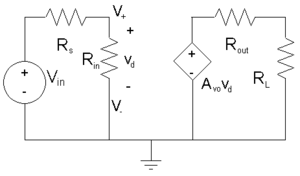
\includegraphics[scale=0.5]{op-amp-model}
                \caption{Op-Amp Model}
                \label{fig:op-amp-model}
            \end{center}
        \end{figure}
        \par An ideal Op-Amp has four characteristics\cite{amp_op_ideal}:
            \begin{quote}
                \begin{itemize}
                    \item Infinite input impedance
                    \item Null output impedance
                    \item Infinite voltage gain
                    \item No limitation at frequency and amplitude response
    
                    \label{list:proprieties}
                \end{itemize}
            \end{quote}
            
        With these proprieties, it is possible to have two basic configurations for an op-amp circuit: virtual short-circuit and virtual mass, as shown below.
        
        \begin{figure}[ht]
            \centering
            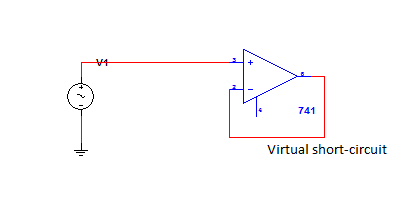
\includegraphics[scale=0.5]{virtual}
            \caption{Virtual short-circuit}
            \label{fig:virtual}
        \end{figure}
        \begin{figure}[ht]
            \centering
            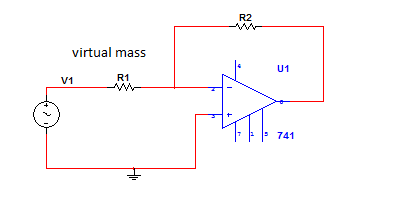
\includegraphics[scale=0.5]{mass}
            \caption{Virtual Mass}
            \label{fig:mass}
        \end{figure}
        As a matter of fact, real op-amps don't have infinite or null values as previously stated, but the values are enough to be considered infinite or zero in calculations. To exemplify this, next table compares values between ideal op-amp and the op-amp used on this project (UA741).
        \begin{table}[h]
            \centering
            \caption{Value difference between ideal and real Op-Amp\cite{amp-op-real}}
            \label{table:amp_op_comp}
            \begin{tabular}{lllll}
                                 & Ideal          & Real        &  & \\
                Gain             & $\infty$       & Over 100000 &  &  \\
                Freq. Response   & Range $ 0$ to $\infty $ & -           &  &  \\
                Input Impedance  & $\infty$       & $2M\Omega $ &  &  \\
                Output Impedance & 0              & $75\Omega $ &  & 
            \end{tabular}
        \end{table}
        \par A summing amplifier can be used as an average amplifier and as as subtractor circuit\cite{summing_amp}. With the use of op-amps, it is also possible to implement a integrator circuit. The integrator circuit implements a Laplace integrator, or, multiplies the input signal by $\frac{1}{s}$\cite{laplace-quote}.
\section{Theoretical Calculations}
    A summing amplifier can be described as the circuit below:
    \begin{figure}[h]
        \centering
        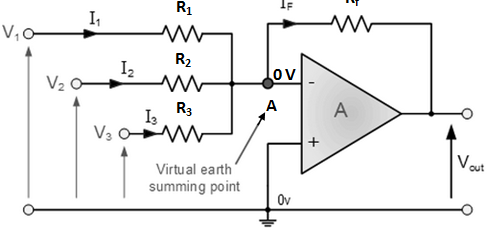
\includegraphics[scale=0.5]{summing}
        \caption{Summing Circuit Topology}
        \label{fig:summing_circ}
    \end{figure}
    \par Once V$_+$ is grounded, then V$_-$ is equal to 0 too, therefore:
        \begin{align}
            V_+ = V_- = 0V \label{math:1}
        \end{align}
    \par As stated before in \ref{list:proprieties}, due to infinite input impedance, current I$_f$ is:
        \begin{align}
            I_f = I_1 + I_2 + I_3 + ... + I_n \label{math:2}
        \end{align}
        Where n is the number of inputs
        And by Ohm's law
        \begin{align}
            V = R.I \label{math:3}
        \end{align}
        Then V$_{out}$ can be written as
        \begin{align}
            V_{out} = -R_fI_f \label{math:4}
        \end{align}
        (The negative sign is due to the inverter input being used)\\
        Substituting~\ref{math:2} on~\ref{math:4} the equation \ref{math:4} can be rewritten as
        \begin{align}
            V_{out} = -R_f (I_1 + I_2 + I_3 + ... + I_n) \label{math:5}
        \end{align}
        Using \ref{math:3} for each input $I_n$
        \begin{align}
            V_{out} =  -R_f (\frac{V_1}{R_1} + \frac{V_2}{R_2} + \frac{V_3}{R_3} + ... + \frac{V_n}{R_n}) \label{math:6}
            \intertext{If $R_f = R_1 = R_2 = R_3 = ... = R_n = R$ then,}
            V_{out} = -(V_1 + V_2 + V_3 + ... + V_n) \label{math:7}
        \end{align}
        Therefore, $V_{out}$ is the sum of the circuit's inputs.
        There are a lot of applications for summing amplifiers, in this project an averager circuit will be implemented,
        where $V_{out}$ is the average of  the inputs.
        \subsection{Average Amplifier}
            For n = 3, there are three inputs on the circuit, as shown\\
            \begin{figure}[h]
                \centering
                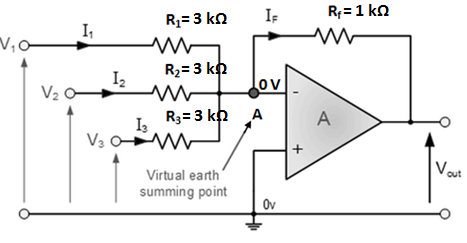
\includegraphics[scale=0.5]{average}
                \caption{Average Summing Circuit}
                \label{fig:average}
            \end{figure}
            \par If we use equation \ref{math:6} we have
            \begin{align}
                V_{out} = -(\frac{Rf}{R1}V1 + \frac{Rf}{R2}V2 + \frac{Rf}{R3}V3) \label{math:8}
            \end{align}
            Since $R_1 = R_2 = R_3 = R$
            \begin{align}
                V_{out} = -\frac{Rf}{R} (V_1 + V_2 + V_3) \label{math:9}
            \end{align}
            For the voltage to be the mean of the inputs, the denominator of $\frac{R_f}{R}$ must be $\frac{1}{n}$, therefore, maintaining order of magnitude of the values, we shall use $R_f = 1k\Omega$ and $R = 3k\Omega$, then \ref{math:9} is:
            \begin{align}
                V_{out} = -(\frac{V_1 + V_2 + V_3}{3}) \label{math:10}
            \end{align}
            The negative sign shows that the phase is the opposite of $V_out$.
        \subsection{Integrator Circuit}
            \par Before assembling an integrator circuit using op-amp, it is important to understand its characteristics:
            A function F(t) is defined as $\frac{F(t)}{dt} = u(t)$, therefore $F(t) = \int u(t) dt$\cite{fundamental-theorem}\cite{laplace-integrator}, in the frequency domain, it can be written as:
            \begin{align}
                sF(s)=U(s) \label{math:11} \\
                F(s)=\frac{U(s)}{s} \label{math:12}
            \end{align}
            \par Which can be interpreted as
            \begin{quote}
                The Laplace transform of an integral is equal to the Laplace transform of the integrand multiplied by $1/s$.\cite{laplace-quote}
            \end{quote}
            \par Then the topology below can be used to implement an integrator.
            \begin{figure}[H]
                \centering
                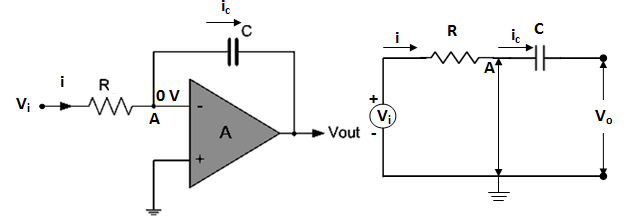
\includegraphics[scale=0.5]{integrator}
                \caption{Integrator Circuit}
                \label{fig:integrator}
            \end{figure}
            \par Demonstration here is very simple, since the impedance at the negative terminal is infinite as stated before \ref{list:proprieties}, then:
            \begin{align}
                i_{in} = i_c \label{math:13}
            \end{align}
            \begin{align}
                i_c = C\frac{dv_c}{dt} \label{math:14}
            \end{align}\\
            But 
            \begin{align}
                v_c = 0 - v_{out} = -v_{out} \label{math:15}
            \end{align}
            and
            \begin{align}
                i_{in} = \frac{v_{in} - 0}{R} = \frac{v_{in}}{R} \label{math:16}
            \end{align}
            Substituting \ref{math:15} in \ref{math:14} and finally \ref{math:14} and
            \ref{math:16} in \ref{math:13}, results in:
            \begin{align}
                \frac{v_{in}}{R} = -C\frac{dv_{out}}{dt} \label{math:17}
            \end{align}
            Integrating both sides:
            \begin{align}
                v_{out} = -\frac{1}{RC}\int \frac{v_{in}}{dt}
            \end{align}
            Therefore, the circuit integrates $V_{in}$ and has a scale of $-\frac{1}{RC}$

\section{Simulation}  
    All the simulations in this project were done in \textit{Multisim} software, this simulator tries to simulate closest possible to reality.
    \subsection{Average Amplifier}
        \subsubsection{DC Case}
            First, an averager circuit was implemented using DC sources. The circuit topology is shown below.
            \begin{figure}[ht]
                \centering
                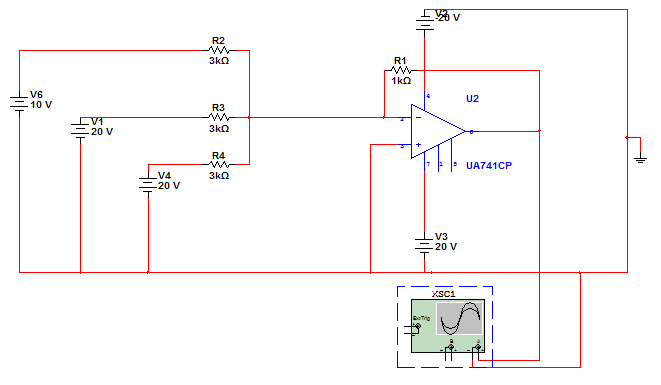
\includegraphics[scale=0.5]{average_simu}
                \caption{Average Amplifier's (DC simulation)}
                \label{fig:average_simu}
            \end{figure}
            \par Analysing the output, it is possible to observe that the voltage is equal to $\frac{1}{3}\sum V_{in}$.
            \begin{figure}[ht]
                \centering
                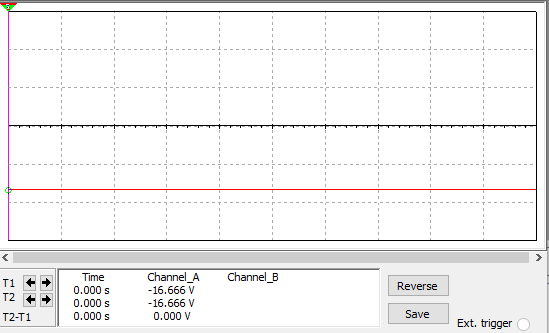
\includegraphics[scale=0.5]{average_result}
                \caption{DC Simulation Output }
                \label{fig:average_result}
            \end{figure}
        
        \subsubsection{AC Case} 
            For the AC case, the following source voltages were used: $V_1 = 2v_{pk}; V_2 = 4v_{pk}; V_3 = 6v_{pk}$.
            \begin{figure}[H]
                \centering
                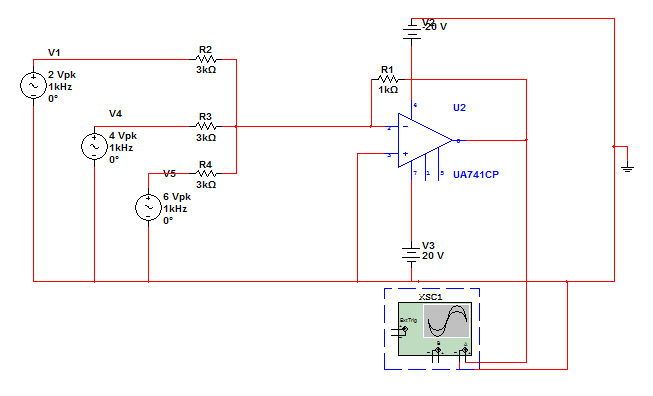
\includegraphics[scale=0.5]{ac_average_simu}
                \caption{Average Amplifier's (AC simulation)}
                \label{fig:my_label}
            \end{figure}
            \begin{figure}[H]
                \centering
                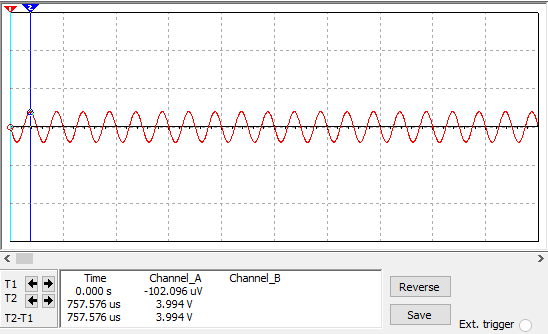
\includegraphics[scale=0.5]{ac_average_result}
                \caption{AC Simulation Output }
                \label{fig:ac_average_result}
            \end{figure}
            \par The expected output is 4V, output acquired was 3.94V, validating the experiment.
    \subsection{Integrator Circuit}
        \par As said before, the integrator circuit integrates an input, and it is possible to see this behavior on oscilloscope output:
        \begin{figure}[H]
            \centering
            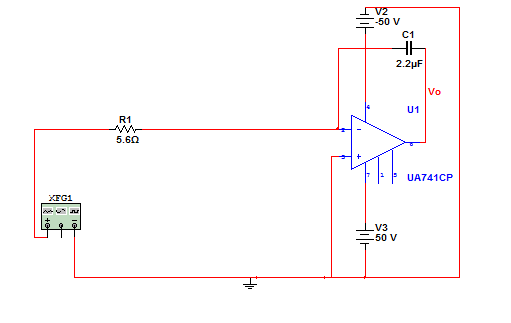
\includegraphics[scale=0.5]{integrator_simu}
            \caption{Integrator Circuit}
            \label{fig:integrator_circuit}
        \end{figure}
        \begin{figure}[H]
            \centering
            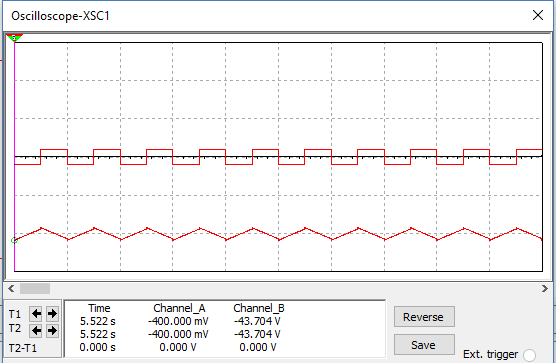
\includegraphics[scale=0.5]{integrator_result}
            \caption{Oscilloscope Output for square wave}
            \label{fig:integrator_result}
        \end{figure}
        \begin{figure}
            \centering
            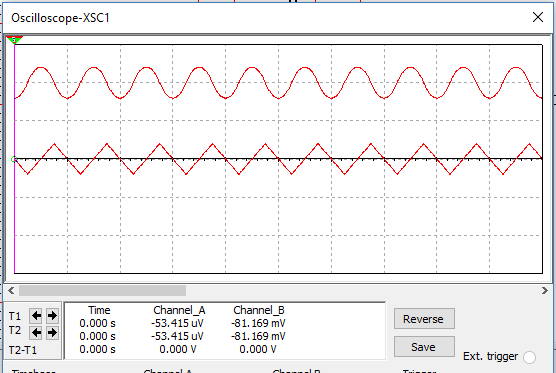
\includegraphics[scale=0.5]{integrator_result2}
            \caption{Oscilloscope Output for triangular wave}
            \label{fig:integrator_result_2}
        \end{figure}{}
        In order to select adequate values for the capacitor and the resistor, it's necessary calculate the RC constant:
        \begin{align}
            \tau=RC={\frac{1}{2\pi f_{c}}} \label{math:19}
        \end{align}
        \par The RC time constant, also called tau, the time constant (in seconds) of an RC circuit, is equal to the product of the circuit resistance (in ohms) and the circuit capacitance.
        \par It is the time required to charge the capacitor, through the resistor, by ≈ 63.2 percent of the difference between the initial value and final value or discharge the capacitor to ≈36.8 percent.\cite{wiki:RC_time_constant}
        \par Once $f_c = \frac{1}{T}$:
        \begin{align}
            RC > \frac{1}{2\pi}T \label{math:20}
        \end{align}
        Then,
        \begin{align}
            RC > 0,16T \label{math:21}
        \end{align}
        The input frequency used was 1KHz, therefore, $T = 1ms$, and finally eq. \ref{math:21} becomes
        \begin{align}
            RC > 0,00016
        \end{align}
        Using a resistor of $5,6K\Omega$ and a capacitor of $2,2\mu F$ yields
        \begin{align}
            RC = 0,01232
        \end{align}
        Satisfying eq. \ref{math:21}.
        \par On the oscilloscope output, it is shown the integrated wave forms, the square wave results in a saw wave and the triangular wave results in a quadratic periodic wave.
\section{Experiment}
    In this section, the experimental results are presented.
    For the averager circuit the following inputs were used: \centerline{$V_1 = 1, V_2 = 2, V_3 = 3$}, the output value on the oscilloscope was 1.88V, and the expected value was 2V, this discrepancy is observed due to inaccuracy of the resistors, but is irrelevant to  the experiment validation.
    \begin{figure}[H]
        \centering
        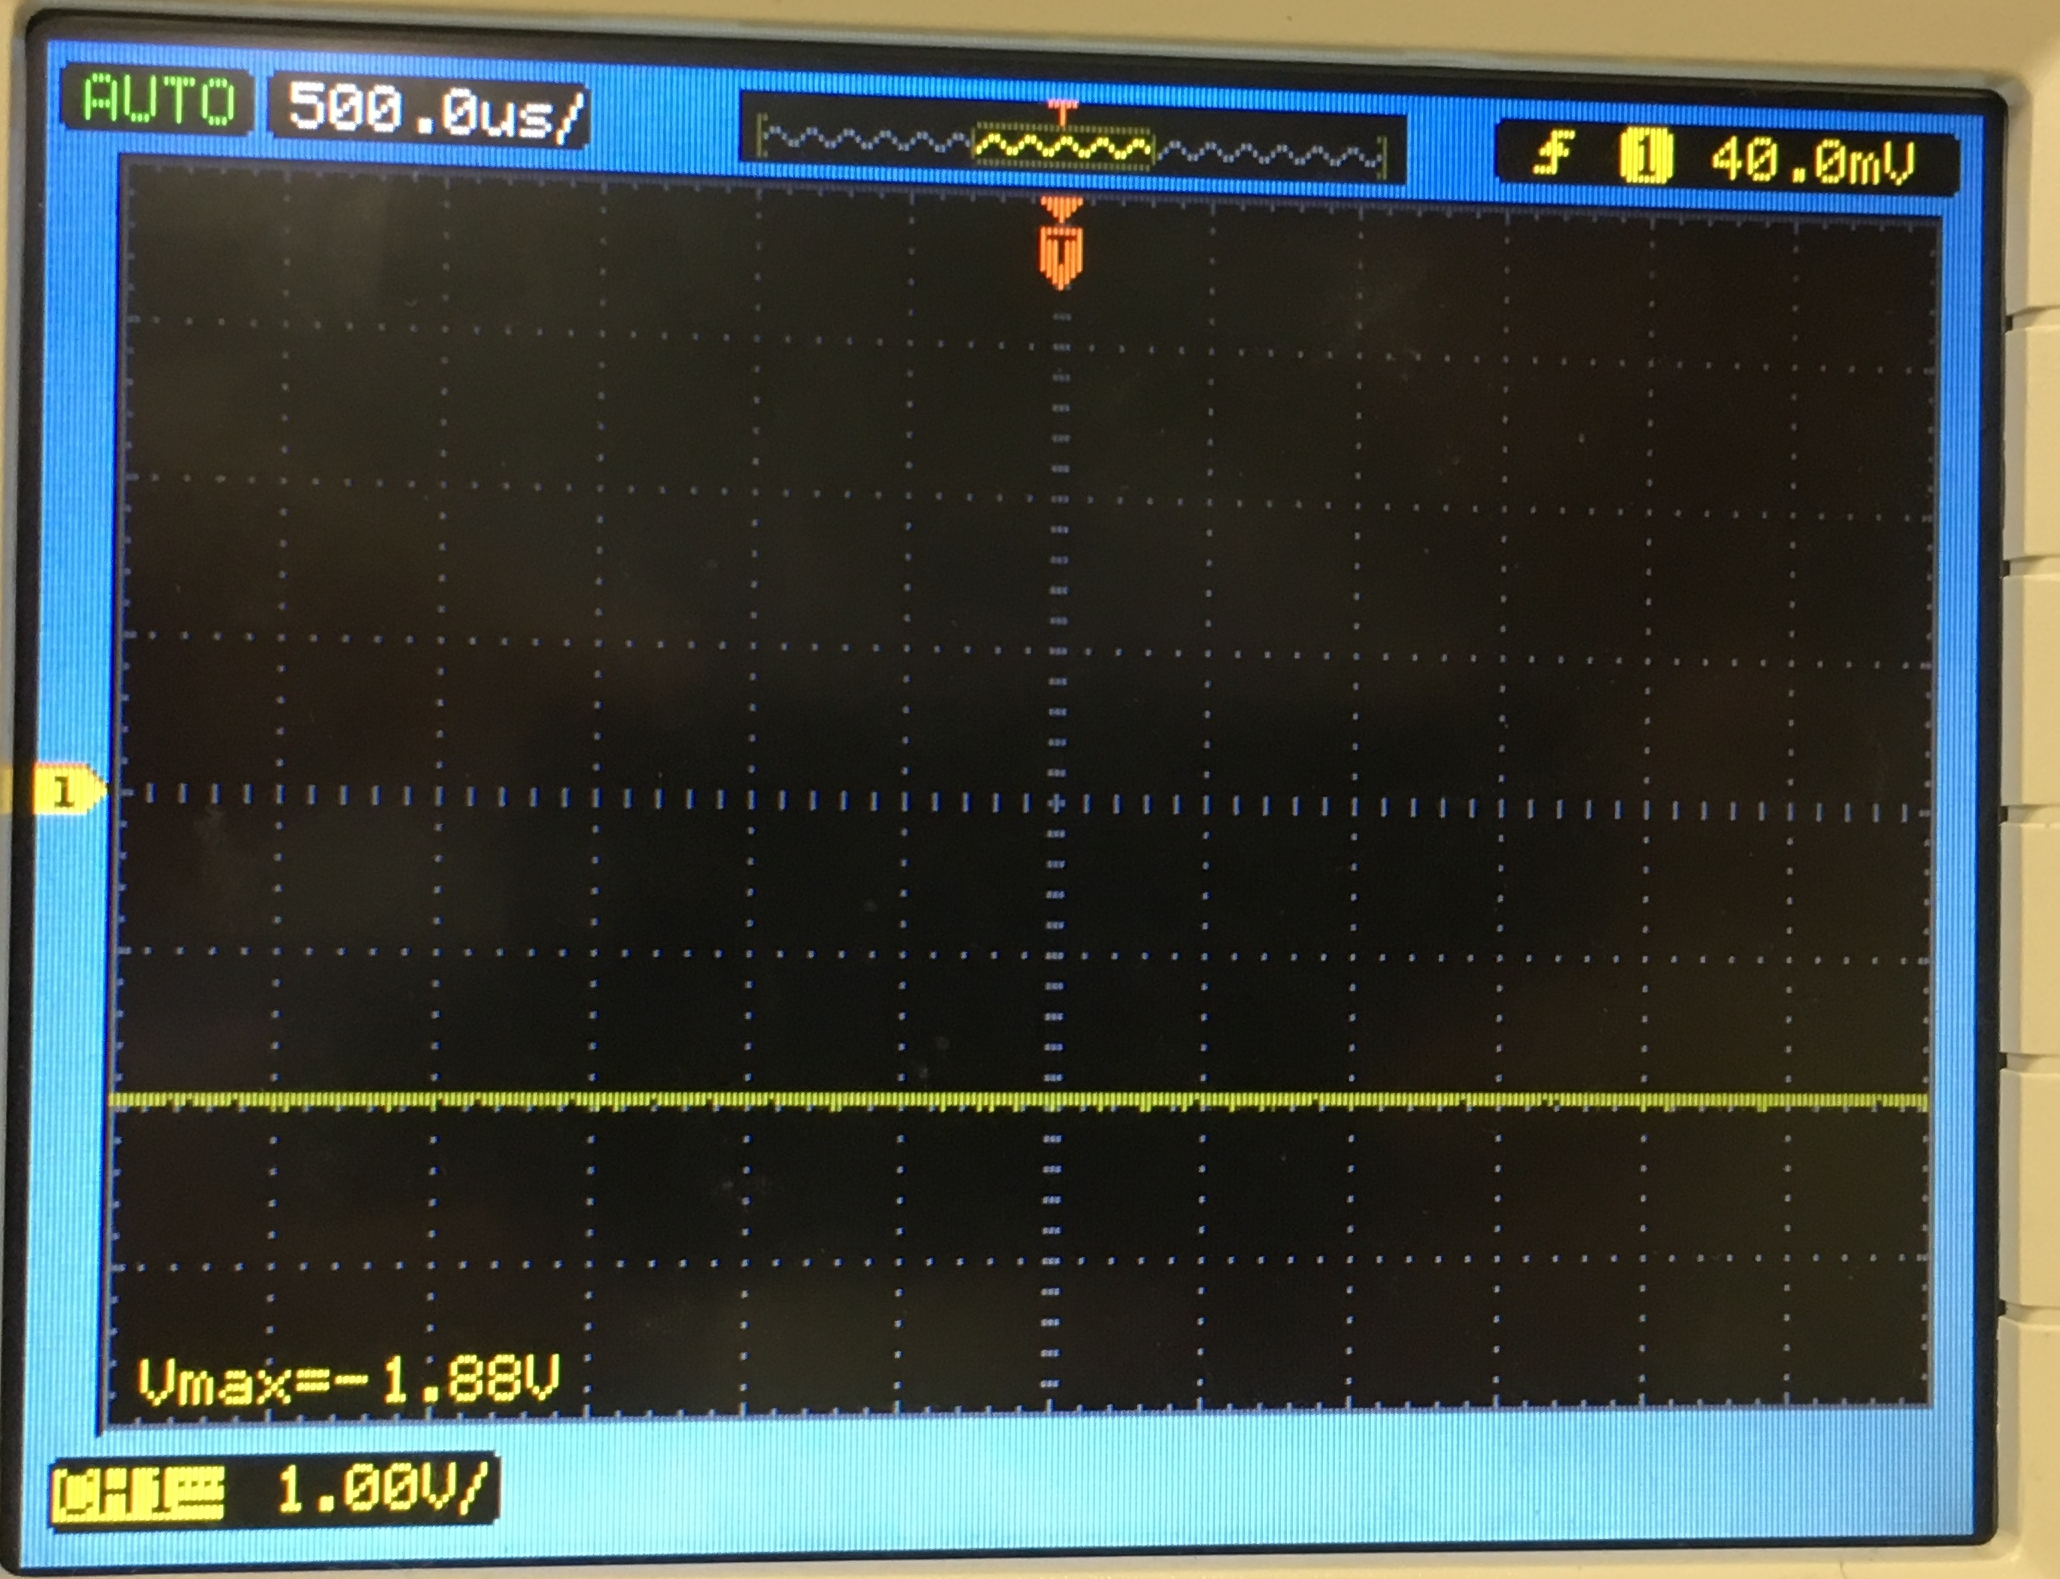
\includegraphics[scale=0.1]{average_real}
        \caption{Output for the implemented averager circuit}
        \label{fig:average_real}
    \end{figure}
    For the second circuit, a square wave was integrated, resulting in a saw wave as expected. The values for the components are the same as used in the presented simulation.
    \begin{figure}[H]
        \centering
        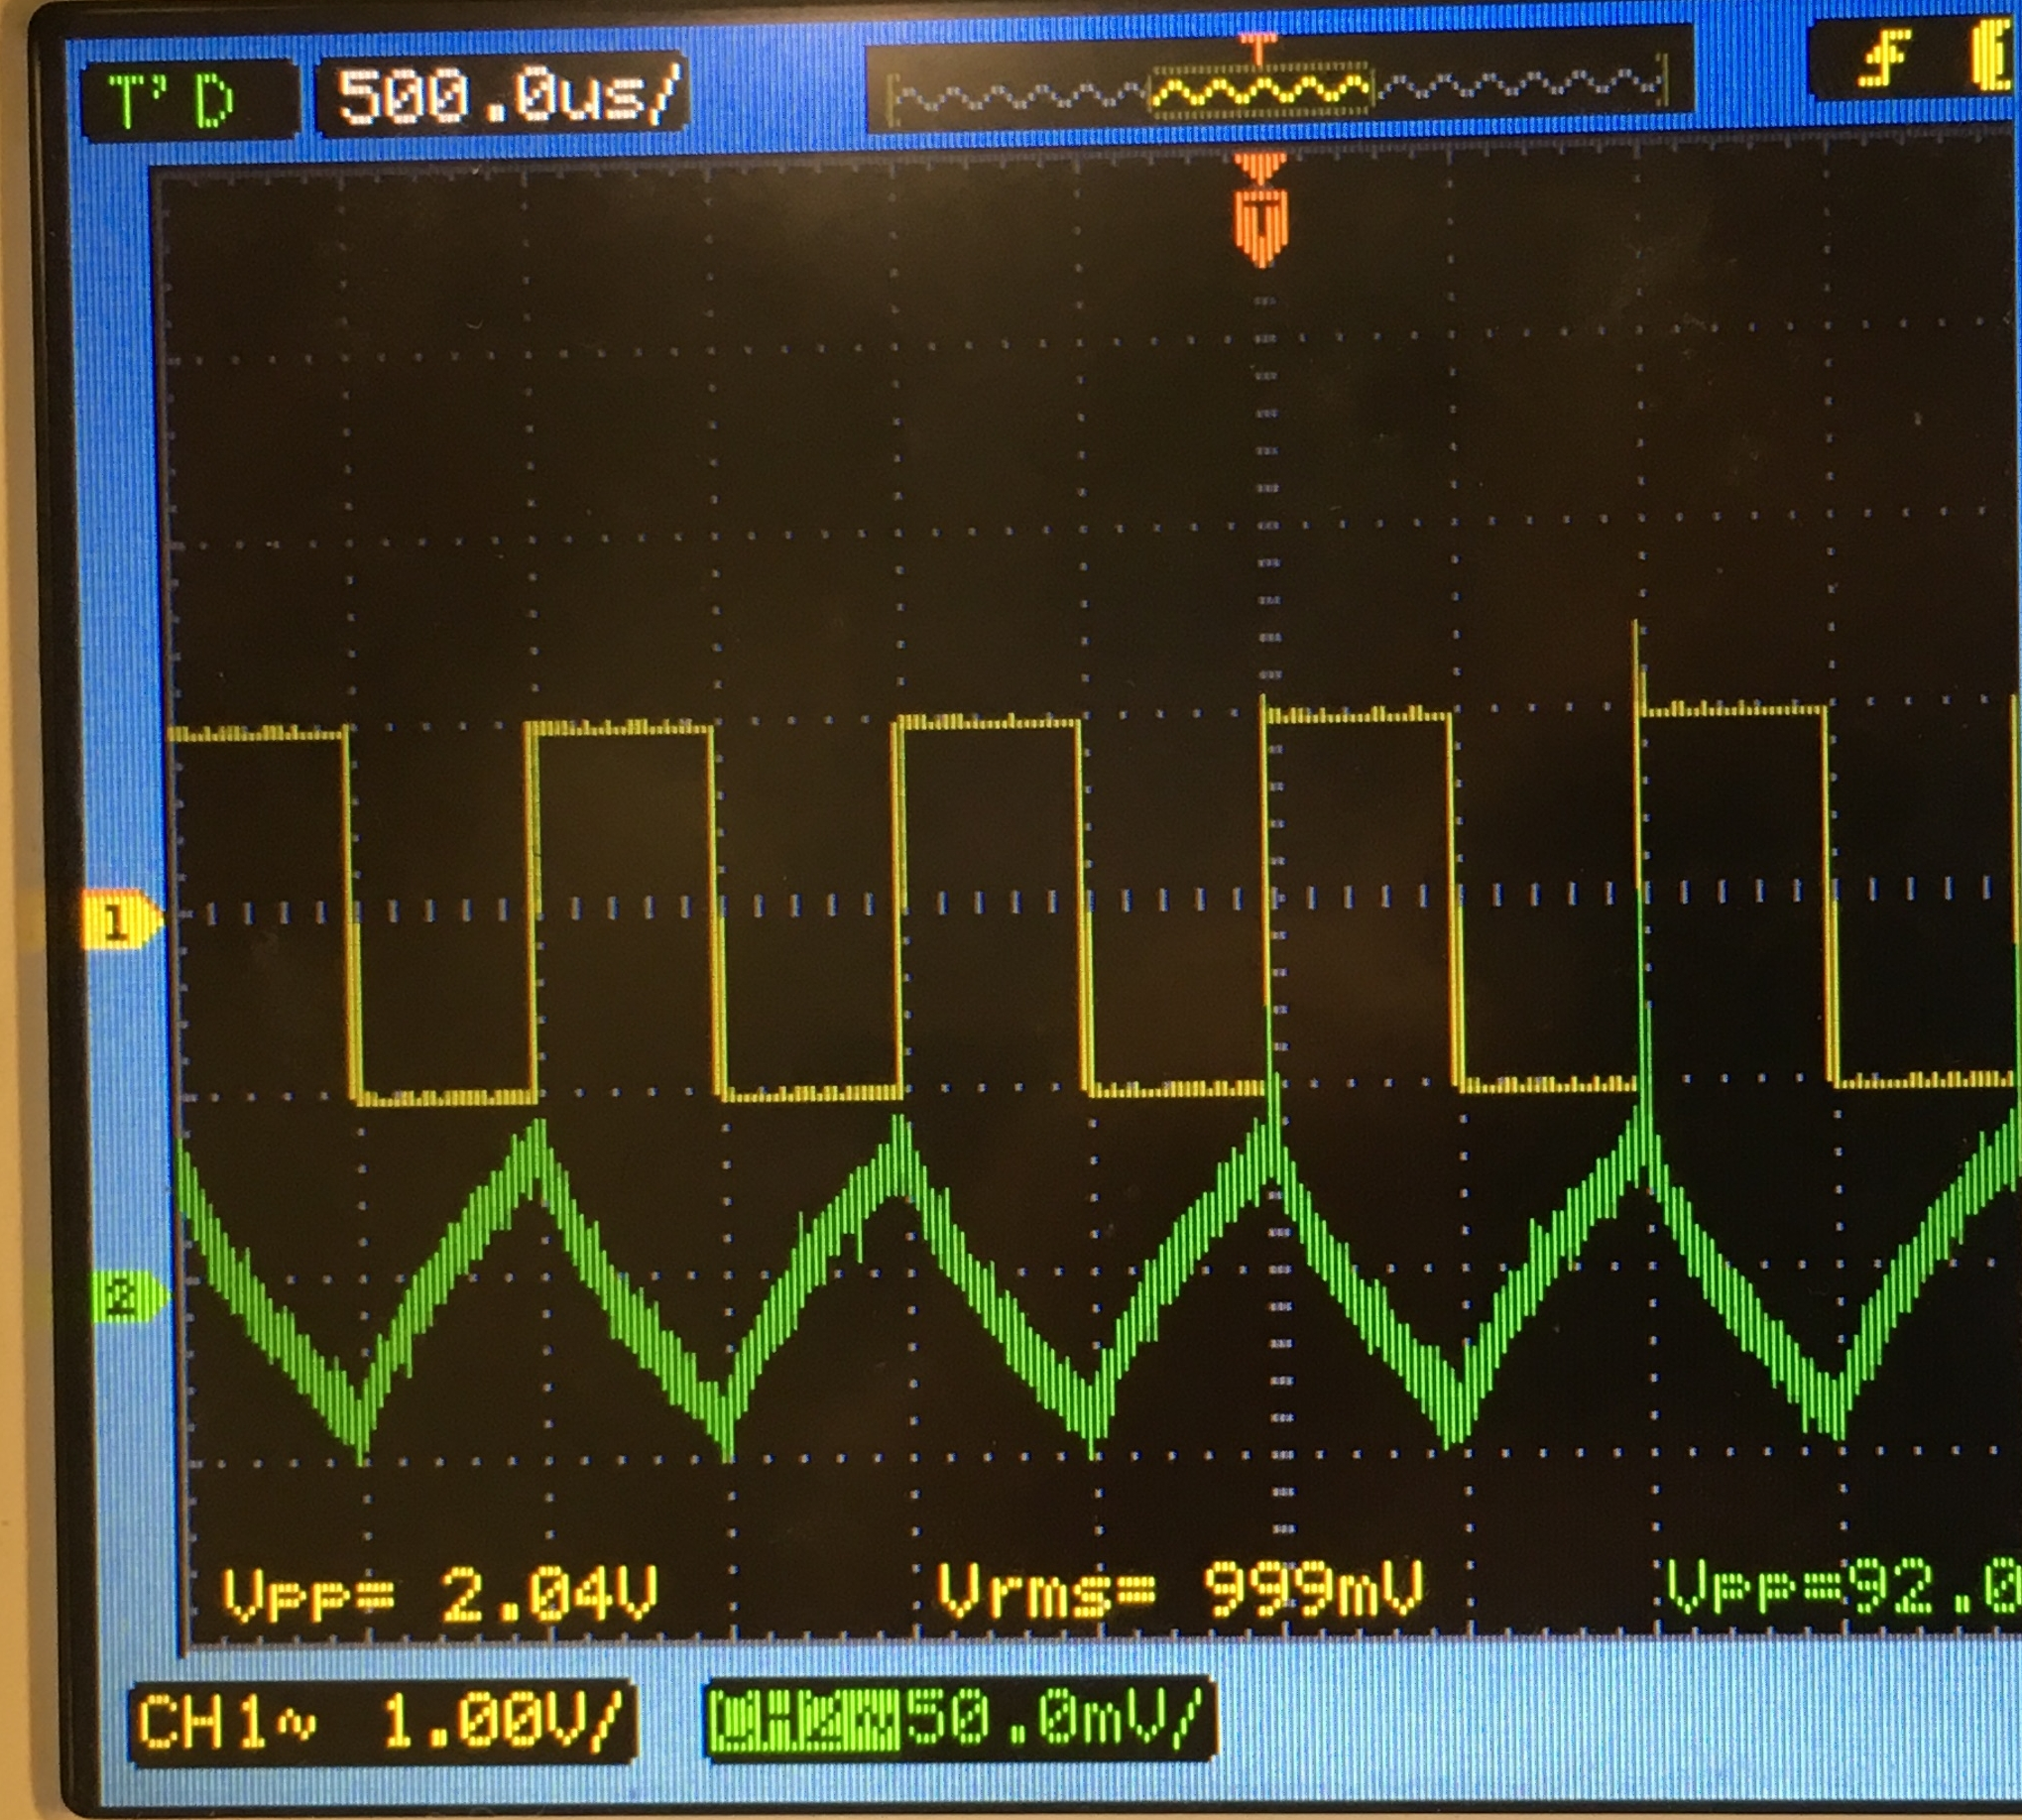
\includegraphics[scale=0.1]{integrator_real}
        \caption{Output for implemented integrator circuit}
        \label{fig:integrator_real}
    \end{figure}
    
\section{Conclusion}
    On this project, expected results were achieved both the DC and AC cases and the modeled circuits can be successfully implemented on a protoboard using op-amps. Real values and theoretical values had insignificant discrepancy and can be considered equal.

\bibliographystyle{IEEEtran}

\bibliography{exemplo}


\end{document}
